\subsection{\label{sec:calib.pol}Beam Polarization}
The electron beam produced with a polarized laser incident on gallium arsenide allows for longitudinal polarization of the electrons~\cite{polarizedelectronsnew} and in turn, due to the bremsstrahlung process, circular polarization of the photon beam.  The accurate measurement of the polarization transferred from the photon beam to the produced hyperons ($C_x$ and $C_z$) requires knowledge of the beam polarization.  Such knowledge is ascertained by knowing the magnitude of incident electron-beam polarization, and the helicity orientation of the electron beam bunch responsible for the event (in the lab-frame). The Maximon-Olsen formula relating incident electron beam polarization, with the photon polarization is given by~\cite{MaximonOlsen},
\begin{equation}
P_\odot(E_\gamma) = \frac{x(4-x)}{4 - 4x + 3x^2}P_{elec}
\end{equation}
where $x = E_\gamma /E_{elec}$ is the ratio of photon energy, $E_\gamma$, to beam energy, $E_{elec}$. The g12 experiment ran with a constant electron energy of $E_{elec} = 5.715$ GeV.  (The actual electron beam energy was corrected on a run-by-run basis, see later section) The polarization of the electron beam was measured regularly using the a M{\o}ller polarimeter.  The polarimeter measures electron polarization by making use of the helicity dependent nature of M{\o}ller scattering~\cite{Mecking,Carman}. The M{\o}ller measurements, summarized in Table~\ref{moltable}, were performed regularly (every few days) during g12 and whenever we were notified of any beam changes. During the g12 running period, Hall B did not have the priority. As a result, the polarization of the beam was delivered as a byproduct as other Halls requirement, and fluctuates. However, the majority of the g12 runs has beam polarization close to 70\% with a total uncertainty estimated to be 5\%.  The run-integrated and flux -weighted value of the polarization of a particular range of photon energies can be easily obtained by using the maximum-Olsen formula.

\begin{table}
\begin{center}

\caption{\label{tab:pol:moller} The degree of longitudinal electron polarization ($P_{e}$) between each M{\o}ller measurements. The uncertainties shown are statistical uncertainties.}

\begin{tabular}{|c|c|}
\hline
Run Range & M{\o}ller Readout ($P_{e}$) \\
\hline 
$56355 - 56475$ & ($81.221 \pm 1.48$)\% \\
\hline 
$56476 - 56643$ & ($67.166 \pm 1.21$)\% \\
\hline 
$56644 - 56732$ & ($59.294 \pm 1.47$)\% \\
\hline 
$56733 - 56743$ & ($62.071 \pm 1.46$)\% \\
\hline 
$56744 - 56849$ & ($62.780 \pm 1.25$)\% \\
\hline 
$56850 - 56929$ & ($46.490 \pm 1.47$)\% \\
\hline 
$56930 - 57028$ & ($45.450 \pm 1.45$)\% \\
\hline 
$57029 - 57177$ & ($68.741 \pm 1.38$)\% \\
\hline 
$57178 - 57249$ & ($70.504 \pm 1.46$)\% \\
\hline 
$57250 - 57282$ & ($75.691 \pm 1.46$)\% \\
\hline 
$57283 - 57316$ & ($68.535 \pm 1.44$)\% \\
\hline

\end{tabular}

\end{center}

\end{table}


An important experimental aspect of g12 is that the electron-beam helicity was flipped at a rate around 30 Hz. While the helicity information was recorded and stored in the HEVT bank for each event, the convention for bit encoding has been known to change from real-time to delayed-time recording. Further considerations, such as the half-wave plate orientation also had to be accounted for.

The only sure way to pin down the absolute beam helicity orientation for our data was to analyze a well known helicity-dependent reaction. Well-established results in Ref.~\cite{Io} in the beam-helicity asymmetry, $I^\odot(\phi^{hel}_\pi)$, for the reaction, $\gamma p \to p \pi^+ \pi^-$, were reproduced.  The mentioned reaction was shown to have a specific helicity-frame defined $\phi^{hel}_{\pi^+}$-dependent structure.  If the helicity convention was reversed then we would observe $I^\odot(\phi^{hel}_{\pi^+}) \to -I^\odot(\phi^{hel}_{\pi^+})$.

The sub-analysis we performed required exclusive $p \pi^+ \pi^-$ events in the final state. To ensure exclusivity we required zero missing energy and momentum within detector resolution. The helicity frame (shown in Fig.~\ref{ioplane}) was defined to be the rest frame of the hypothetical parent meson of the two pion system, with  $\hat{z}$ aligned along its center-of-mass defined momentum. $\phi^{hel}_{\pi^+}$ is the angle between the proton-production plane, and the plane containing both pions. The beam helicity asymmetry is given by,
\begin{equation}
I_\odot = \frac{1}{P_{\gamma}} \frac{N^+ - N^-}{N^+ + N^-},
\end{equation}
where $N^\pm$ indicates the number of events with positive (negative) photon helicity.  Figs.~\ref{myIo}-\ref{Io} show the $I_{\odot}(\phi^{hel}_{\pi^+})$ for g12 and in the analysis of \cite{Io}.
The lab-frame electron helicity readout was taken from the HEVT bank (HEVT$\to$hevt[0].TGRPRS). The results of our $I_{\odot}(\phi^{hel}_{\pi^+})$ analysis and the previously published results showed a positive (negative) HEVT readout indicates positive (negative) photon helicity. The following method, stored in\begin{verbatim} /work/clas/clasg12/clasg12/clas6-trunk/include/gethelicity.h \end{verbatim} takes care of these issues and returns the helicity for a given event:

\begin{verbatim}
int GetHelicity(clasHEVT_t *HEVT)
{
     int helicity = 0;
     int readout = HEVT->hevt[0].trgprs;
     if(readout > 0) helicity = 1;
     if(readout < 0) helicity = -1;
     return helicity;
}
\end{verbatim}

The reproduction of beam-helicity asymmetry for double charged pion production also served as a way to test the accuracy of the calculated photon polarization magnitude: both results' wave amplitudes were in good agreement. 
FIU and FSU independently measured the beam-helicity asymmetry and were in good agreement with each other. The pull distribution between FIU and FSU is shown in figure~\ref{fig:pol:g12compare} and the pull distribution between FIU and g1c's results are shown in figure~\ref{fig:pol:g12g1ccompare}. Both FIU and FSU use approximately 15\% of the entire dataset (due to the independence of the two measurements, their selection of the data is most likely not the same). Figure~\ref{fig:pol:g12g1ccompare} shows good agreement between g12 and g1c's beam-helicity measurement.


\begin{figure}[htpb]
\begin{center}
 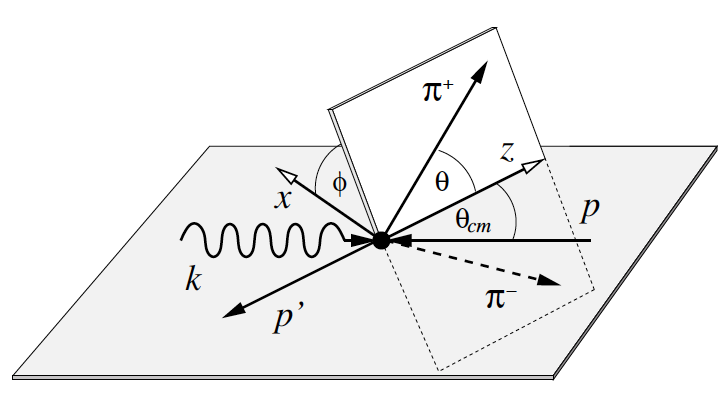
\includegraphics[width=0.4\columnwidth]{{figures/calib/pol/ioplane}.eps}
  \caption{\label{ioplane}An illustration of the angle definitions used in the $\gamma p \to \pi^+ \pi^- p$ sub-analysis. $\theta_{cm}$ is defined in the center-of-mass frame. $\theta$ and $\phi$ are defined in the rest frame of the $\pi^+$ $\pi^-$ system as the polar and azimuthal angles. The $z$ direction is along the total momentum of the $\pi^+ \pi^-$ system.}
  \end{center}
\end{figure}


\begin{figure}[htpb]
\begin{center}
  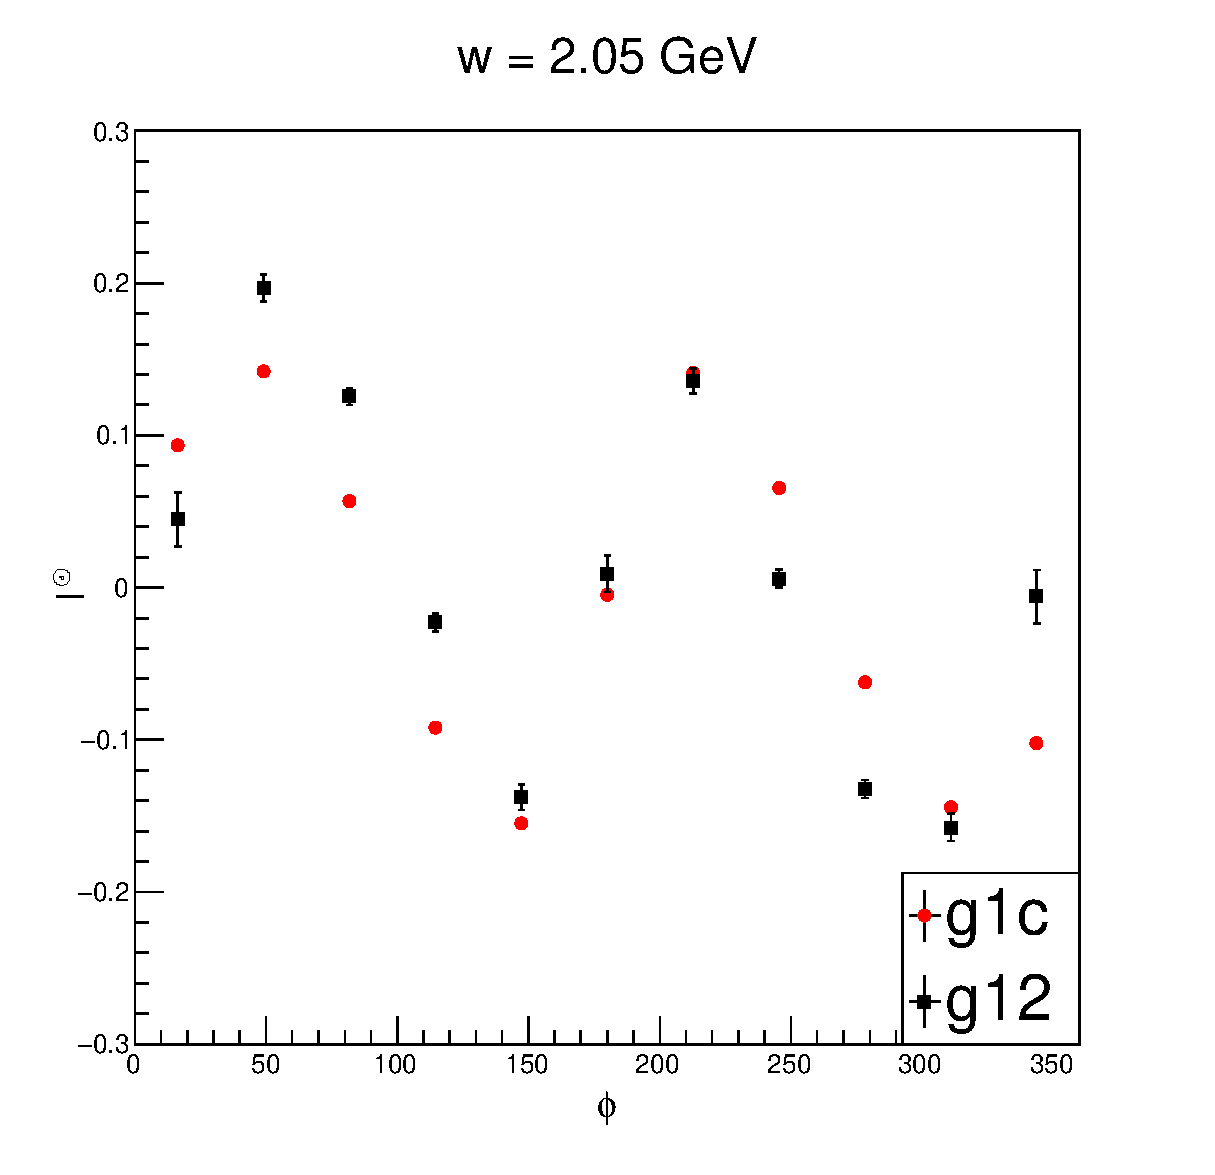
\includegraphics[width=0.4\columnwidth]{{figures/calib/pol/iodotcompare}.eps}
  \caption{\label{myIo}$I_{\odot}(\phi^{hel}_{\pi^+})$ comparison between g12 (FIU) and g1c within the energy range $W = 2.05 \pm .025$ GeV.}
  \end{center}
\end{figure}


\begin{figure}[htpb]
\begin{center}
 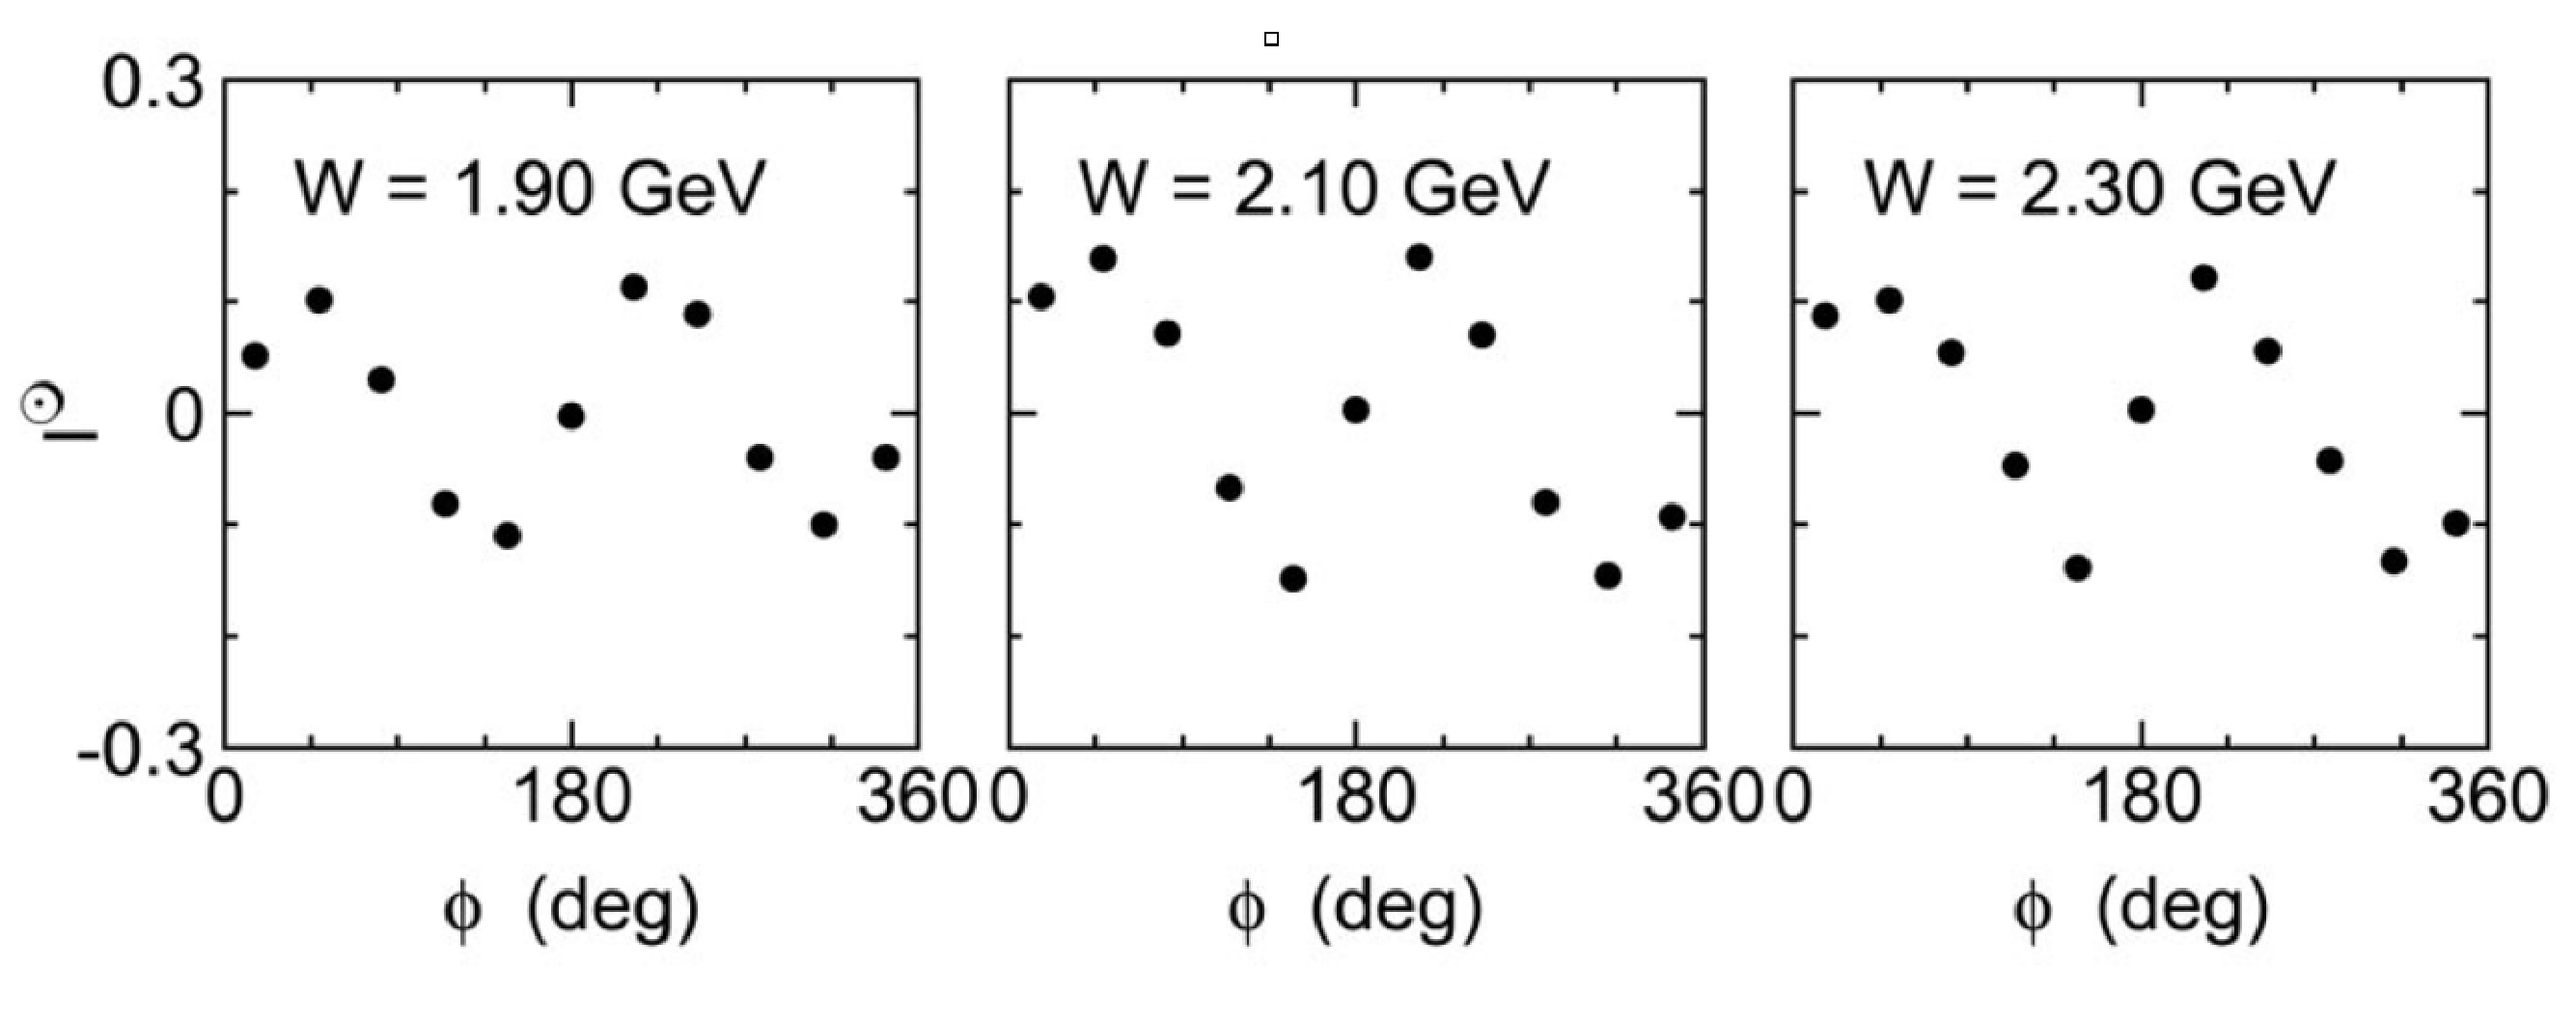
\includegraphics[width=0.8\columnwidth]{figures/calib/pol/Io.eps}
  \caption{\label{Io}$I_{\odot}(\phi^{hel}_{\pi^+})$ as measured in the previous analysis.}{ $I_{\odot}(\phi^{hel}_{\pi^+})$ as measured in the analysis~\cite{Io}. The results of are shown in bins of $W$ from 1.9 to 2.3 GeV.}
  \end{center}
\end{figure}

\begin{figure}[htpb]
\begin{center}
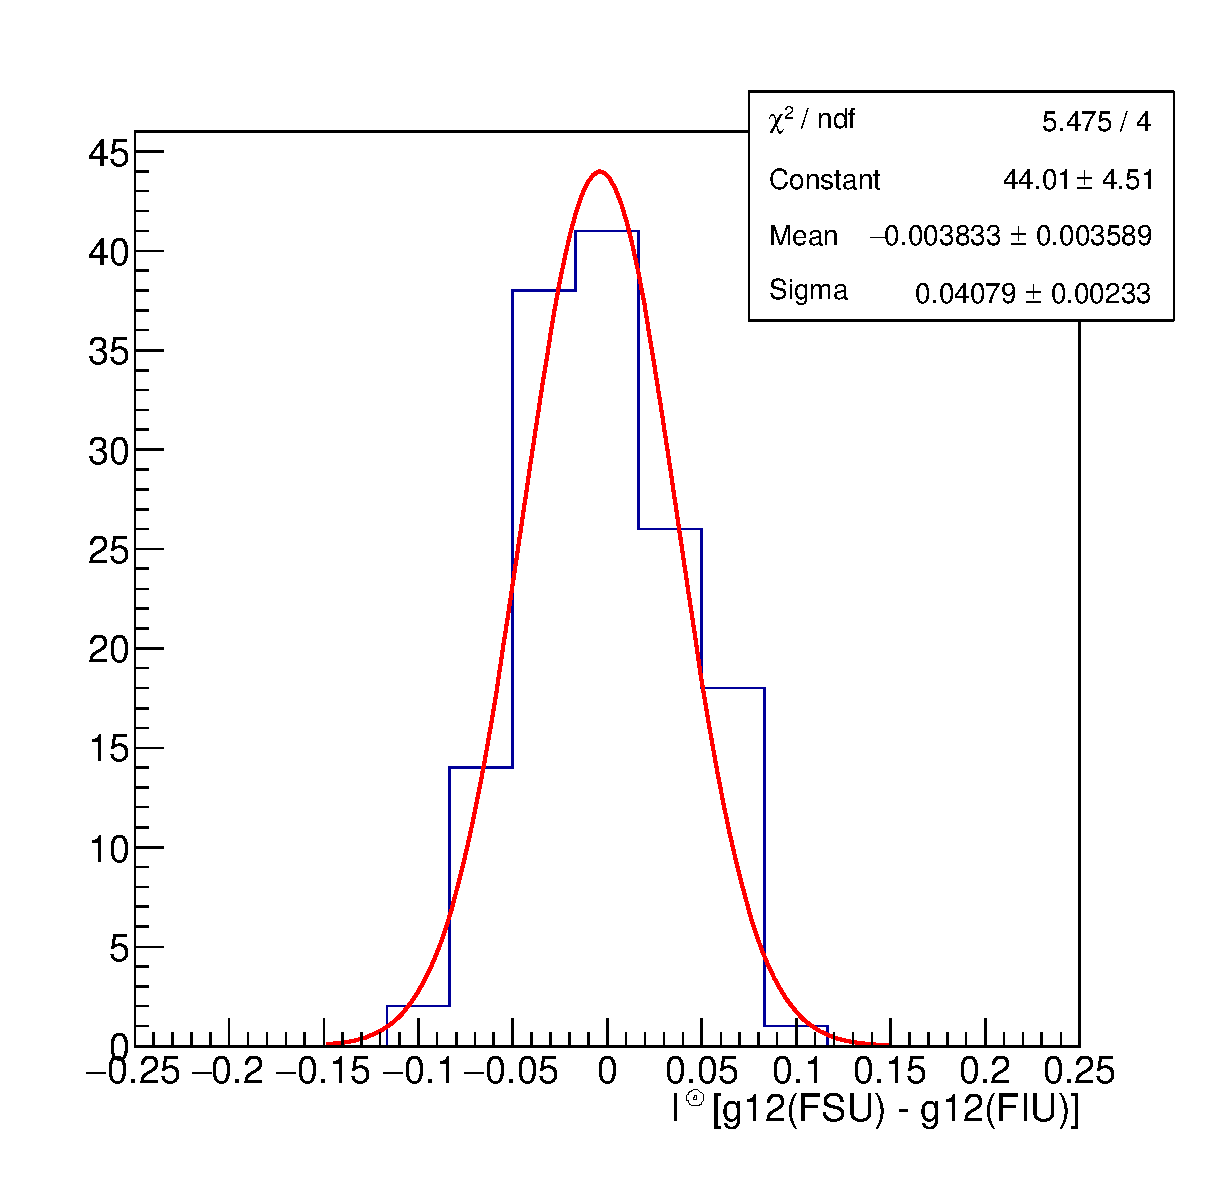
\includegraphics[width=0.4\columnwidth]{{figures/calib/pol/g12compare}.eps}
\caption{\label{fig:pol:g12compare} Pull distribution between FIU and FSU $I^{\odot}$ }
\end{center}
\end{figure}

\begin{figure}[htpb]
\begin{center}
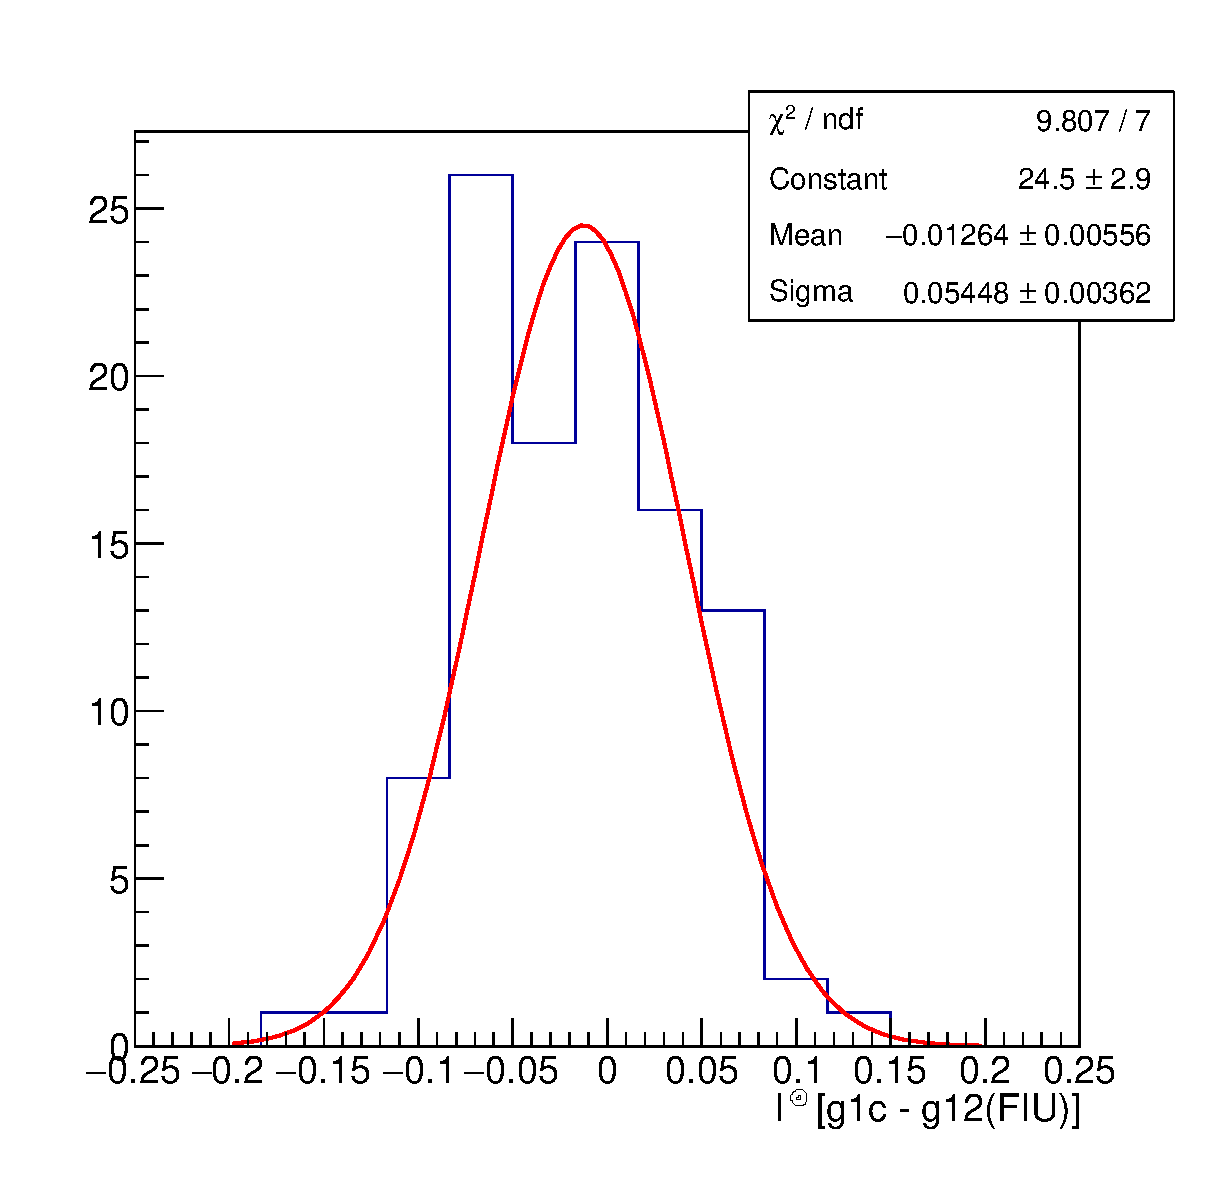
\includegraphics[width=0.4\columnwidth]{{figures/calib/pol/g12g1ccompare}.eps}
\caption{\label{fig:pol:g12g1ccompare} Pull distribution between g12 (FIU) and g1c $I^{\odot}$ }
\end{center}
\end{figure}

To conclude, the g12 beam polarization was measured with standard methods, and the validity of the photon helicity definition in the HEVT bank was double checked against existing experimental results and confirmed to be correct. All g12 measurements that utilizes the beam polarization refer to what has been summarized here.


